% Intended LaTeX compiler: xelatex
\documentclass[a4paper, 12pt]{article}
\usepackage{graphicx}
\usepackage{longtable}
\usepackage{wrapfig}
\usepackage{rotating}
\usepackage[normalem]{ulem}
\usepackage{amsmath}
\usepackage{amssymb}
\usepackage{capt-of}
\usepackage{hyperref}
\usepackage[danish]{babel}
\usepackage{mathtools}
\usepackage[margin=3.0cm]{geometry}
\hypersetup{colorlinks, linkcolor=black, urlcolor=blue}
\setlength{\parindent}{0em}
\parskip 1.5ex
\author{Jacob Debel}
\date{Fysik B}
\title{Eksperimenter med bevægelse i én (og/eller to) dimension(er)\\\medskip
\large Mekanik}
\hypersetup{
 pdfauthor={Jacob Debel},
 pdftitle={Eksperimenter med bevægelse i én (og/eller to) dimension(er)},
 pdfkeywords={},
 pdfsubject={},
 pdfcreator={Emacs 29.4 (Org mode 9.6.15)}, 
 pdflang={Danish}}
\begin{document}

\maketitle


\section*{Indledning}
\label{sec:org72befda}
\begin{center}

\includegraphics[width=7cm]{img/2019-12-10_07-58-00_film-and-vid.jpg}
\end{center}

Fysik indeholder som bekendt både skriftlige, mundtlige og eksperimentelle aspekter. 
Fokus er i denne omgang på det mundtlige aspekt. For i stedet for at producere klassiske fysikrapporter skal der indspilles og afleveres \textbf{videoprodukter}. Yderligere skal I også selv designe og udføre eksperimenterne.

\section*{Gruppearbejde}
\label{sec:orga8f1ac8}
I skal inddeles i mindre grupper af 3 eller 4 elever. I bestemmer selv, hvordan I vil fordele jer.

\section*{Emner}
\label{sec:org3dc9a1a}
\begin{center}
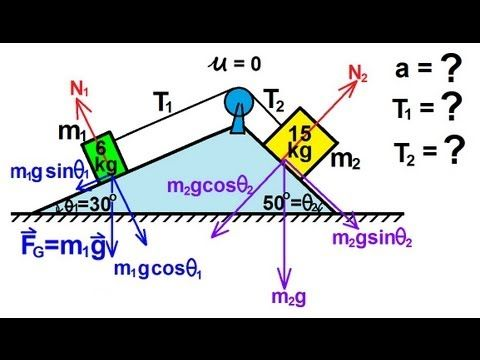
\includegraphics[width=7cm]{img/2019-12-10_07-41-43_34817502643b8a0b0805dd422c8a8283.jpg}
\end{center}

I løbet af undervisningen i translatorisk mekanik har vi blandt andet arbejdet med følgende emner:
\begin{itemize}
\item bevægelse med konstant hastighed.
\item bevægelse med konstant acceleration.
\item (t,s)-, (t,v)- og (t,a)-grafer.
\item Lodret kast (og lidt med det skrå kast).
\item Newtons love.
\item forskellige typer af kræfter: snorkræfter, fjederkræfter/Hookes lov, opdrift, friktion og luftmodstand.
\item Arbejde og energi.
\item potentiel energi, kinetisk energi og mekanisk energi.
\item energi oplagret i en fjeder.
\end{itemize}

\newpage

\section*{Design af eksperimenter}
\label{sec:orgffcc7ef}
\begin{center}
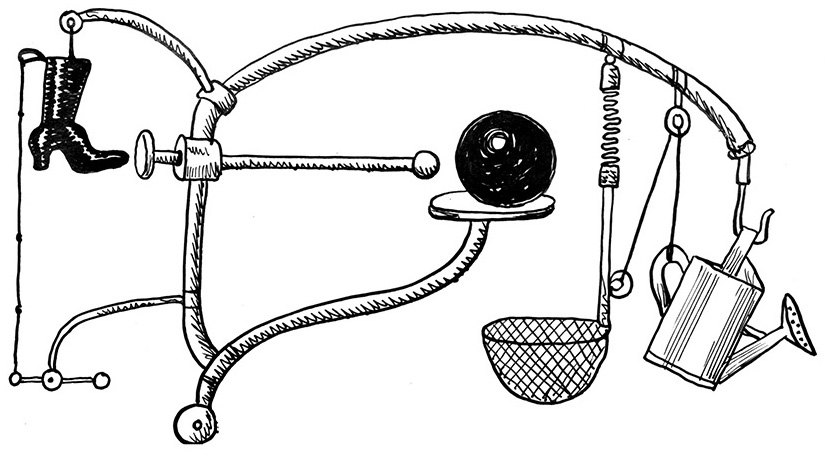
\includegraphics[width=7cm]{img/2019-12-10_07-37-00_vandekandedimstilweb2.jpg}
\end{center}

I skal i jeres grupper selv designe og udføre et eller flere eksperimenter som kan belyse et godt udvalg af de førnævnte emner. Om det skal være ét stort forkromet eksperiment eller flere simple, er op til jer.

Hvis man ikke selv kan komme på nogle gode eksperimenter, kan man blive inspireret af følgende liste:
\begin{itemize}
\item Undersøgelse af det frie fald.
\item Fald med luftmodstand.
\item Et lodret kast.
\item Et lodet kast med vindmodstand (semisvært).
\item Det skrå kast.
\item Det skrå kast med vindmodstand (svært).
\item Bestemmelse af friktionskoefficienter mellem selvvalgte materialer.
\item Undersøgelse af statiske og dynamiske friktionskoefficienter.
\item Undersøgelse af forskellige fjedre og Hookes lov.
\item Undersøgelse af elastikker eller andre fjedrende materialer, og om de opfører sig efter Hookes lov.
\item (Lodret) skud med slangebøsse. Byg den selv.
\item Acceleration af vogne og lodder på en skinne.
\item Bevægelser på et skråplan. (Er i 2 dimensioner, så det er for dem, som gerne vil udfordres).
\end{itemize}

\newpage

\section*{Krav til videoerne}
\label{sec:org8b386f5}
Der skal være særligt fokus på den \textbf{teoretiske} beskrivelse af forsøget og fysikken (formlerne) bag, men også på præsentation af \textbf{resultaterne efter datahandling}. Videoerne skal derfor indeholde:
\begin{itemize}
\item En præsentation af eksperimenterne, og hvilke størrelser der ønskes bestemt i dem.
\item En analyse af eksperimenterne. Det kunne f.eks. være at indtegne kræfter på en figur og finde den resulterende kraft og efterfølgende vise de beregninger/udledninger med symboler, som skal til for at bestemme en værdi for de ønskede størrelser.
\item En \emph{kort} forklaring på, hvilke målinger der skal foretages i eksperimenterne, og hvordan disse udføres.
\item En uddybende præsentation af resultaterne efter databehandlingen. Selve databehandlingen skal der ikke bruges synderlig meget tid på. Den skal gerne give sig selv, efter man har set analyserne af eksperimenterne.
\end{itemize}

Der er selvfølgelig frihed til indsætte andre indslag i videoerne, hvis det vil fremme formidlingen.

Videoerne må maksimalt have en varighed på \textbf{10 minutter} i deres endelige form.

\section*{Gode råd til videoindspilning}
\label{sec:orgf7d70f6}
\begin{itemize}
\item Udarbejd en drejebog (storyboard på engelsk). Hvilke scener skal der være med.
\item Overvej, hvordan videoerne skal indspilles. Screencast på computeren, live foran kameraet, en blanding eller måske noget helt andet. Alle gruppemedlemmer skal dog præsentere noget i videoen.
\item Overvej, hvilke former for rekvisitter, som skal være med. Det kan både være fysiske og elektroniske.
\item Øv jer på jeres replikker, udledninger osv. inden selve indspilningen. Min egen erfaring er, at jeg altid skal øve mig mindst tre gange, før end en vigtig præsentation sidder lige i skabet.
\end{itemize}
\end{document}
